\begin{figure} \centering
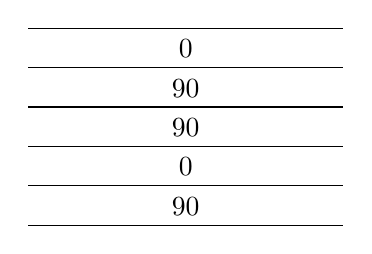
\begin{tikzpicture}
	\draw (0,0) -- (4,0);
	\draw (0,-0.5) -- (4,-0.5) node[midway, above] {$0$};
	\draw (0,-1) -- (4,-1) node[midway, above] {$90$} ;
	\draw (0,-1.5) -- (4,-1.5) node[midway, above] {$90$};
	\draw (0,-2) -- (4,-2) node[midway, above] {$0$};
	\draw (0,-2.5) -- (4,-2.5) node[midway, above] {$90$};
\end{tikzpicture}
\caption{Model for cross ply laminate}
\end{figure}
